\chapter{Nawigacja}\label{chap:naw}

    Kluczowym dla gry założeniem jest ułatwienie graczowi wczucia się w realia świata, w którym się znajduje. Jako jeden z głównych warunków pogłębienia immersji uwypuklono brak implementacji mapy, na której gracz widziałby świat. W ten sposób nie upraszczamy mu poruszania się i odnajdywania lokacji tak, jak i człowiek w realnym świecie w czasach średniowiecznych nie kierował się zapisanymi na kartce kartograficznymi obrazami, ale własną i zdobytą od innych wiedza o otaczającym go terenie. 
    Jedyną pomocą, jaką otrzyma gracz, będzie pasek obrazujący pole widzenia granej postaci. Pierwszą rolą narzędzia będzie pokazanie kierunku świata, który znajduje się w polu widzenia gracza. Zakładamy, że grana postać potrafi sama taką, informację odczytać chociażby z położenia Słońca. Nie jest to więc sztucznie upraszczająca rozgrywkę mechanika, a jedynie odciążenie użytkownika kompasem. 
    Kolejną informacją na omawianym polu będzie miejsce w którym znajduje się przeciwnik. Dotyczy to antagonistów widocznych w polu widzenia, jak i ukrytych za ścianą. Druga część będzie logicznie możliwa dzięki specjalnej umiejętności widzenia wrogów za przeszkodą zaimplementowanej dla postaci druida. Po przyłączeniu takiej osoby do drużyny użytkownik może poprosić przyjaciela o użyczenie mu swej mocy.

\begin{figure}[htbp]
    \centering
    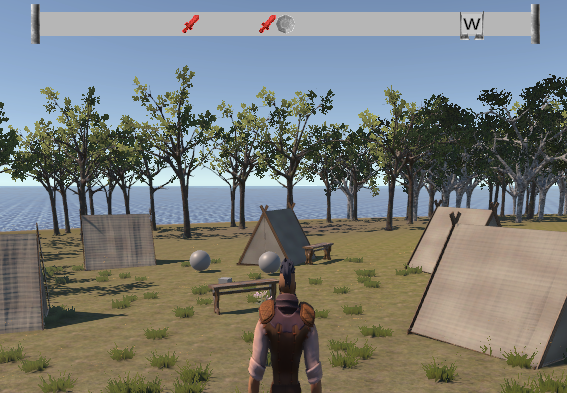
\includegraphics[width=0.9\textwidth]{images/ui/compass.png}
    \caption{Wizualizacja przypadku, w którym gracz patrzy centralnie na północ. Delikatnie na jego prawo znajduje się dwóch przeciwników za ściana, podświtlonych specjalną umiejętnościa druida.
    }\label{fig:compass}
\end{figure}

